\documentclass[10pt]{beamer}

\usetheme{metropolis}
\useoutertheme{metropolis}
\useinnertheme{metropolis}
\usefonttheme{metropolis}
%\usecolortheme{seahorse}   % or your preferred color theme
\usepackage{appendixnumberbeamer}
\usepackage{graphicx}
\usepackage{booktabs}
\usepackage[scale=2]{ccicons}
\usepackage{xspace}
\usepackage[justification=centering]{caption}

\usepackage[version=3]{mhchem}
\definecolor{darkgreen}{RGB}{30, 133, 12}
\definecolor{lightgray}{gray}{0.9}
\renewcommand{\arraystretch}{1.2}

\title{Hartree-Fock Stability}
\subtitle{Applications to the Homogeneous Electron Gas \\ And Implications in Electron Correlation}
\date{\today}
\author{Evan Curtin}
\institute{University of Illinois at Urbana-Champaign}
\titlegraphic{\hfill
\includegraphics[height=1.5cm]{../images/imark_bold.eps}}

\begin{document}

\maketitle

\begin{frame}{Table of contents}
  \setbeamertemplate{section in toc}[sections numbered]
  \tableofcontents[hideallsubsections]
\end{frame}

\section{Background Information}

{%
\setbeamertemplate{frame footer}{Seeger, R.; Pople, J. A. J. Chem. Phys. 1977, 66 (7), 3045.
}
\begin{frame}[fragile]{Levels of Hartree-Fock Theory}
	\begin{center}
		\begin{tabular}{ | c | c | c | c |}
			\hline
			 \textbf{Method} & \textbf{Spinorbital} & \textbf{DoF} & \textbf{Eigenfunction of}\\ 
			\hline 

			Restricted \rule{0pt}{7ex} & 
			\begin{tabular}{c@{}c@{}}				
				$\chi_j^\alpha(\vec{r},\sigma) = 
				\sum\limits_{i=1}^{N} c_{ij}\phi_i\left(\vec{r \,}\right)\alpha(\sigma)$
				\\ \rule{0pt}{4ex} 
				$\chi_j^\beta(\vec{r},\sigma) =
				\sum\limits_{i=1}^{N} c_{ij}\phi_i\left(\vec{r \,}\right)\beta(\sigma)$
			\end{tabular}
			& N/2 
			& $\hat{S}^2$, $\hat{S}_z$
			\\ [5ex] \hline
			
			Unrestricted \rule{0pt}{7ex} &
			\begin{tabular}{c@{}c@{}}  
			$\chi_j^\alpha(\vec{r},\sigma) = \sum\limits_{i=1}^{N} 
			c_{ij}^\alpha\phi_i(\vec{r \,}) \alpha(\sigma)$
			\\ \rule{0pt}{4ex}
			$\chi_j^\beta(\vec{r},\sigma) = \sum\limits_{i=1}^{N} 
			c_{ij}^\beta\phi_i(\vec{r \,}) \beta(\sigma)$
			\end{tabular}
			& N & $\hat{S}_z$ \\ [5ex]
			\hline 
			
			General \rule{0pt}{7ex}&
			\begin{tabular}{r@{}r@{}}  
				$\chi_j(\vec{r},\sigma) = \sum\limits_{i=1}^{N} [
				c_{ij}^\alpha\phi_i\left(\vec{r \,}\right) \alpha(\sigma) $
				\\ \rule{0pt}{4ex}
				$+c_{ij}^\beta \phi_i(\vec{r \,}) \beta(\sigma)]  $
			\end{tabular} 
			& 2N & Neither \\ [5ex]
			\hline			
		\end{tabular}
	\end{center}
\end{frame}

{%+
\setbeamertemplate{frame footer}{}


\begin{frame}[fragile]{Restricted Minimization}
	\begin{itemize}
		\item<1-> Hartee-Fock SCF guarantees only stationary energy w.r.t. change in orbitals
		\item<1-> The solution may be a maximum, minimum or saddle point
		\begin{itemize}
			\item<2->[] \begin{alertblock}{Within the Constrained Space} \end{alertblock}
		\end{itemize}
	\end{itemize}
	\begin{center}
		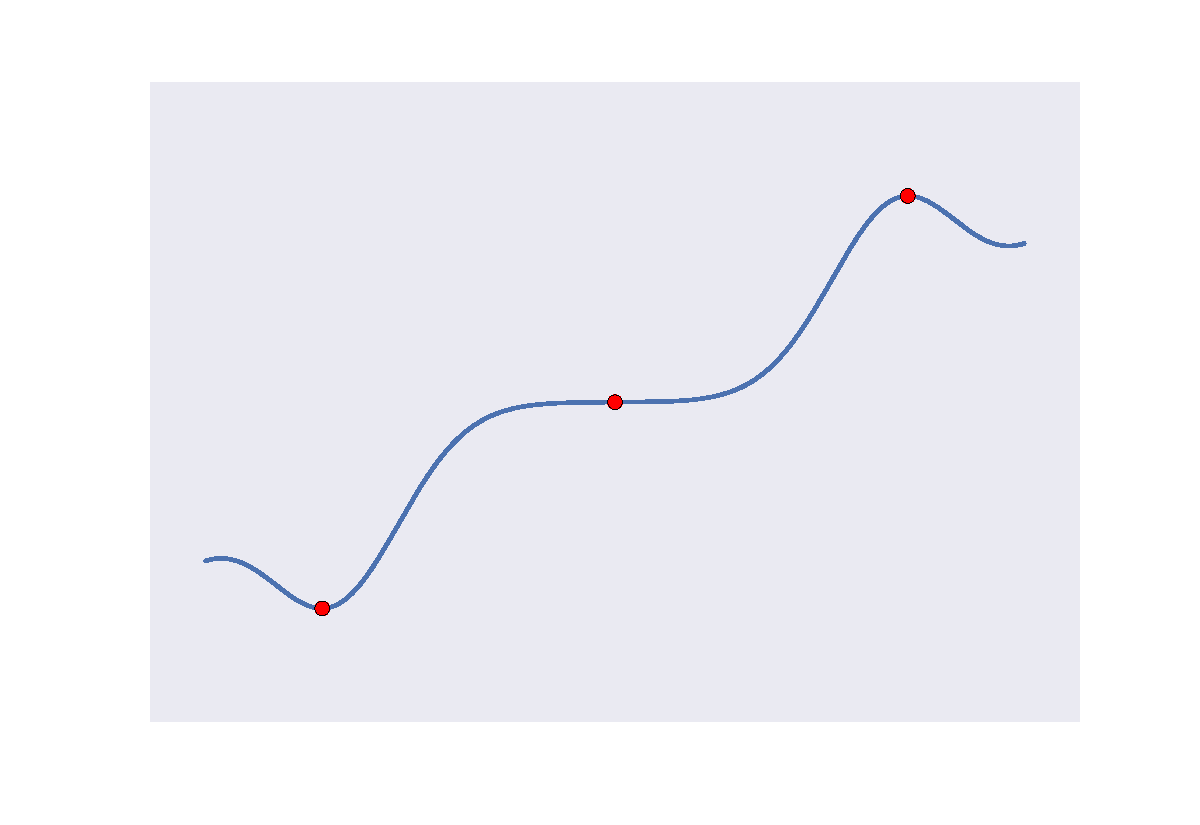
\includegraphics[width=0.5\textwidth, trim={3cm, 2cm, 3cm, 2cm}, clip]{../images/1d_extrema.pdf}
	\end{center}
\end{frame}

\begin{frame}{Restricted Minimization}
	\begin{columns}[c] % align columns
		\begin{column}{.48\textwidth}
			\begin{itemize}[<+->]
				\item {Restricted minima may correspond to absolute minima}
				\item {Restricted minima may correspond to absolute maxima}
				\item {Restricted minima may be nonstationary}
			\end{itemize}				
		\end{column}
		\hfill
		\begin{column}{0.48\textwidth}
		    \begin{overprint}
			    \onslide<1>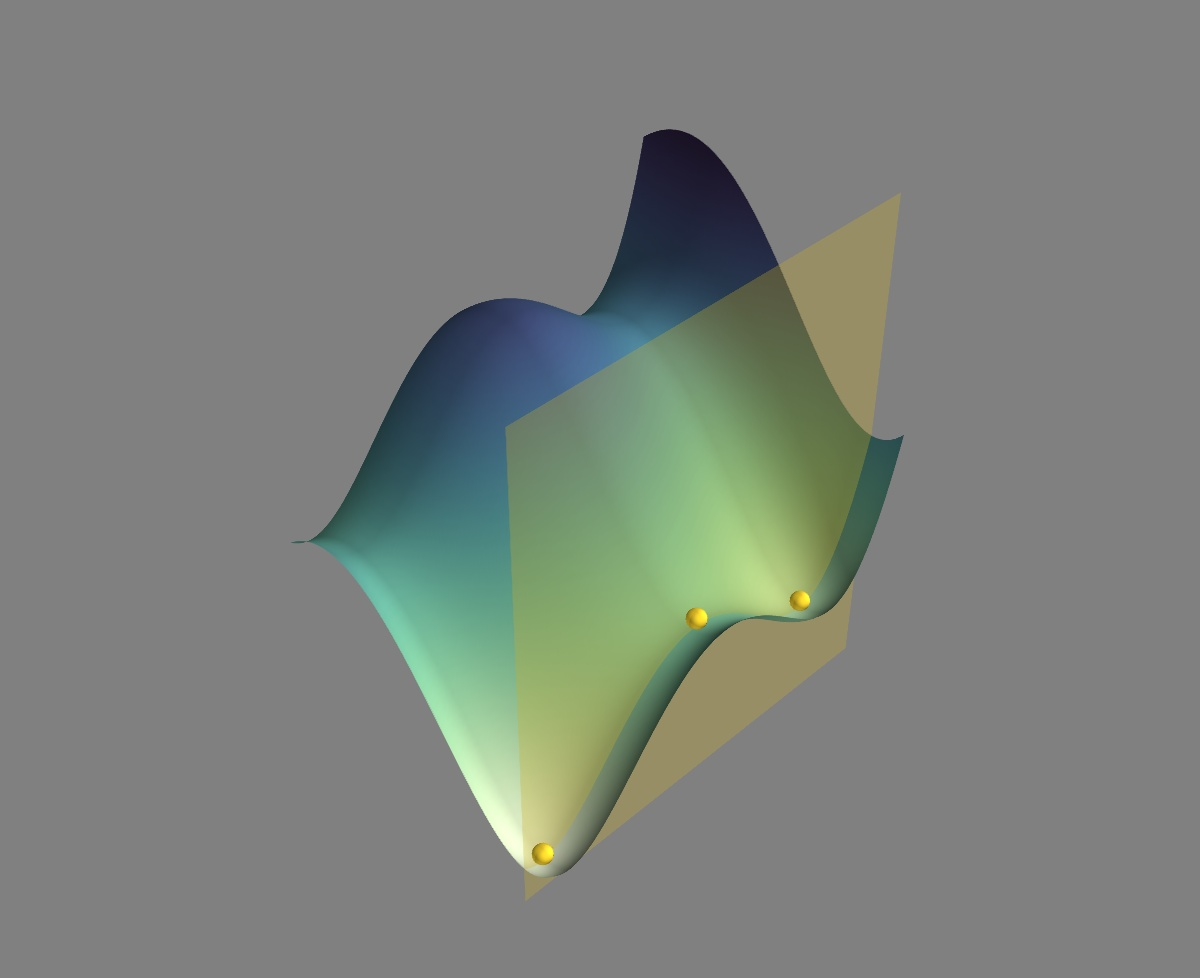
\includegraphics[width=0.9\linewidth, trim={7cm, 2cm, 7cm, 3cm}, clip]{../images/const_opt_globalmin.jpeg}
				\onslide<2>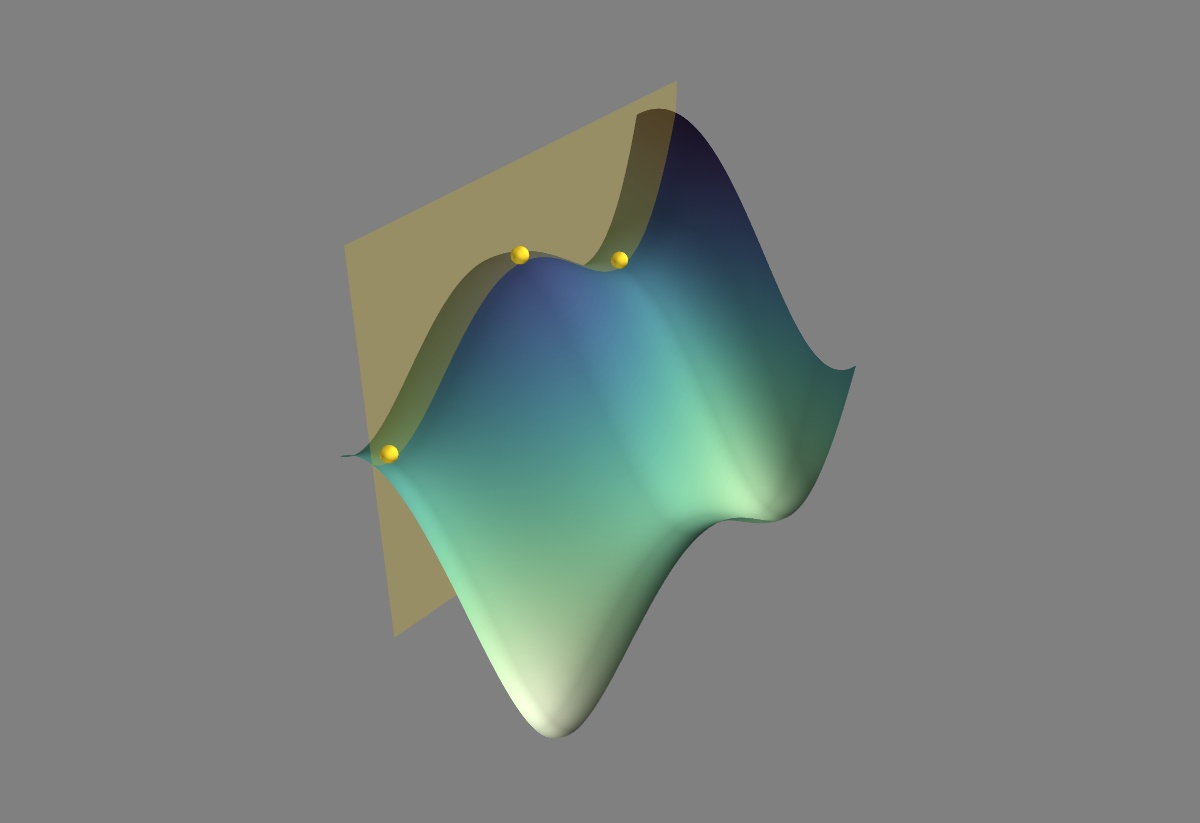
\includegraphics[width=0.9\linewidth, trim={7cm, 1cm, 7cm, 1cm}, clip]{../images/const_opt_saddle.jpeg}
				\onslide<3>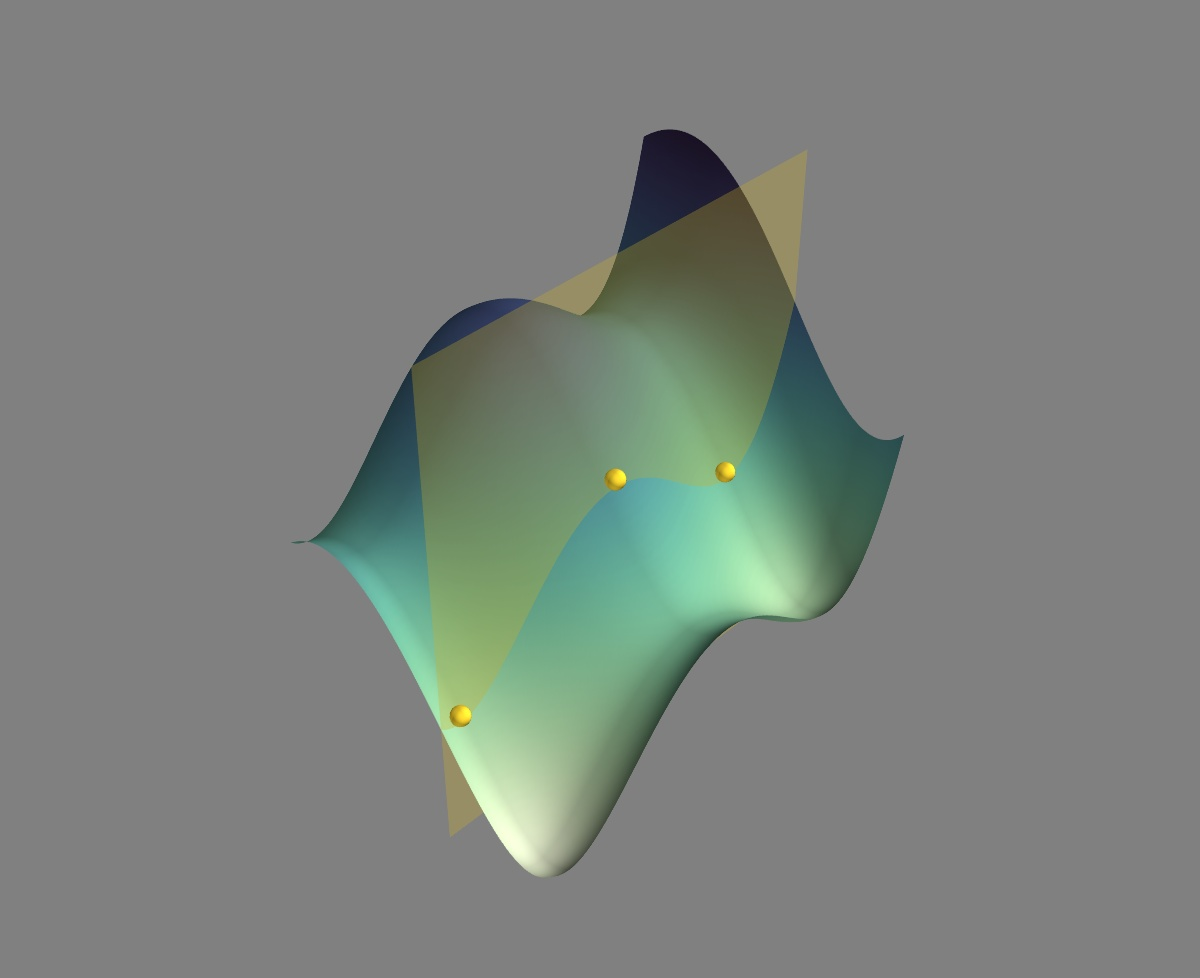
\includegraphics[width=0.9\linewidth, trim={7cm, 2cm, 7cm, 3cm}, clip]{../images/const_opt_nonstationary.jpeg}
			\end{overprint}
		\end{column}	
	\end{columns}
\end{frame}

\section{Hartree-Fock Stability}

{%
	\setbeamertemplate{frame footer}{Thouless, D. J. Nucl. Phys. 1960, 21, 225–232.}
\begin{frame}{Outline}
	\begin{columns}[c] % align columns
		\begin{column}{.48\textwidth}
			\begin{itemize}
				\item {Inspired by biological evolution}
				\item {Evolve a population over generations}
				\item {Survival of the fittest}
				\item {Requirements:}
				\begin{itemize}
					\item {Represent individuals as vector}
					\item {Fitness function}
				\end{itemize}
				\item{$v = \left(\begin{smallmatrix}
					x_1 & y_1 & z_1 & x_2 &  y_2 & z_2 &
					... & x_N & y_N & z_N
					\end{smallmatrix}\right)$}
				\item{$F = \frac{E_{max} - E}{E_{max} - E_{min}}$}
			\end{itemize}

		\end{column}
		\hfill
		\begin{column}{0.48\textwidth}

		\end{column}	
	\end{columns}
\end{frame}
}

{%
\setbeamertemplate{frame footer}{1. Supady, A.; Blum, V.; Baldauf, C. J. Chem. Inf. Model. 2015, 55 (11), 2338–2348.
		
2. http://www.chemspider.com/Chemical-Structure.2298795.html}
\begin{frame}{From Structure to Vector}
	\begin{columns}[c] % align columns
		\begin{column}{.48\textwidth}
			\begin{itemize}
				\item<1-> {Several Ways to Define Structure
					\begin{itemize}
						\item[] {Cartesian}
						\item[] {Internal Coordinates (bond length, angle ...)}
						\item[] {SMILES, InChI}
					\end{itemize}
				}
				\item<2-> {InChI$^2$= 1S/C8H16/c1-5-7(3)8(4)6-2/h5-6H2,1-4H3/b8-7-}
				\item<only@3> {Equivalent in theory}
				\item<only@4> {Equivalent \alert{\textbf{in theory}}}
			\end{itemize}			
		\end{column}
		\hfill
		\begin{column}{0.48\textwidth}
			1
		\end{column}	
	\end{columns}
\end{frame}
}


\begin{frame}{Selecting Parents}
	\begin{columns}[c] % align columns
		\begin{column}{.48\textwidth}
			\begin{itemize}[<+->]
				\item {Several methods are common}
				\item {Reinforce good characteristics}
				\item {Still give losers a chance}
				\item {'Breed' pairs of winners}
				\item {'Roulette Wheel' Method}
			\end{itemize}				
		\end{column}
		\hfill
		\begin{column}{0.48\textwidth}

		\end{column}	
	\end{columns}
\end{frame}

{%
\setbeamertemplate{frame footer}{http://www.turingfinance.com/computational-finance
	
-updates-ieee-world-congress-computational-intelligence}
\begin{frame}{The Next Generation}
	\begin{itemize}[<+->]

		\item[]{~\\Crossover distinguishes this from Monte Carlo}
	\end{itemize}
\end{frame}
}


\begin{frame}{The Whole Algorithm}
	\begin{columns}[c] % align columns
		\begin{column}{.48\textwidth}
			\begin{itemize}[<+->]
				\item[1.] {Generate N random, sensible geometries}
				\item[2.] {Add each to blacklist}
				\item[3.] {Optimize each geometry}
				\item[4.] {Select Parents}
				\item[5.] {Crossover \& Mutate into sensible geometry}
				\item[6.] {Add Children to population}
				\item[7.] {Remove High energy individuals}
				\item[8.] {If converged:}
				\begin{itemize}
					\item{Done!}
				\end{itemize}
				\item[] {Otherwise:}
				\begin{itemize}
					\item{Go to 2}
				\end{itemize}
			\end{itemize}
		\end{column}
		\hfill
		\begin{column}{0.48\textwidth}
			\onslide<11>\begin{itemize}
				\medskip
				\item[]{

				}
			    \item[]{

				}
			\end{itemize}
		\end{column}	
	\end{columns}
\end{frame}

\section{Finding Low Energy Conformers of Dipeptides}

{%
	\setbeamertemplate{frame footer}{Supady, A.; Blum, V.; Baldauf, C. J. Chem. Inf. Model. 2015, 55 (11), 2338–2348.}
\begin{frame}{Dipeptide Structures}

\end{frame}
}

{%
\setbeamertemplate{frame footer}{Supady, A.; Blum, V.; Baldauf, C. J. Chem. Inf. Model. 2015, 55 (11), 2338–2348.
}
\begin{frame}{Combinatorics}
	\begin{columns}[c] % align columns
		\begin{column}{.4\textwidth}
			\begin{itemize}
				\item {GA beats other methods if space is large}
				\item {Space gets large \textbf{\alert{fast}}}
			\end{itemize}		
		\end{column}
		\hfill
		\begin{column}{0.6\textwidth}

		\end{column}	
	\end{columns}
\end{frame}
}

{%
\setbeamertemplate{frame footer}{Supady, A.; Blum, V.; Baldauf, C. J. Chem. Inf. Model. 2015, 55 (11), 2338–2348.
}
\begin{frame}{Coverage}
	\begin{columns}[c] % align columns
		\begin{column}{.4\textwidth}
			\begin{itemize}
				\item {Smaller systems are reliably sampled}
				\item {As \# of conformers increases, miss more and more}
				\item {Is there a pattern to what is missed?}
			\end{itemize}		
		\end{column}
		\hfill
		\begin{column}{0.6\textwidth}

		\end{column}	
	\end{columns}
\end{frame}
}

{%
\setbeamertemplate{frame footer}{Supady, A.; Blum, V.; Baldauf, C. J. Chem. Inf. Model. 2015, 55 (11), 2338–2348.
}
\begin{frame}{Coverage}
	\begin{columns}[c] % align columns
		\begin{column}{.4\textwidth}
			\begin{itemize}[<+->]
				\item {Most misses are very high energy}
				\item {Algorithm favors low energy areas of the space}
				\item {Features low in energy are favored and recombined}
			\end{itemize}		
		\end{column}
		\hfill
		\begin{column}{0.6\textwidth}

		\end{column}	
	\end{columns}
\end{frame}
}

{%
\setbeamertemplate{frame footer}{Supady, A.; Blum, V.; Baldauf, C. J. Chem. Inf. Model. 2015, 55 (11), 2338–2348.}
\begin{frame}{Energy Cutoff}
	\begin{columns}[c] % align columns
		\begin{column}{.4\textwidth}
			\begin{itemize}[<+->]
				\item[] {

				}
				\item {GA is more sensitive to energy cutoff}
				\item {For finding low energy ensemble, GA outperforms purely stochastic/deterministic method}
			\end{itemize}		
		\end{column}
		\hfill
		\begin{column}{0.6\textwidth}

		\end{column}	
	\end{columns}
\end{frame}
}

\section{Concluding Remarks}

{%
\setbeamertemplate{frame footer}{Supady, A.; Blum, V.; Baldauf, C. J. Chem. Inf. Model. 2015, 55 (11), 2338–2348.}
\begin{frame}{Concluding Remarks}
	\begin{itemize}[<+->]
		\item {Finding all the low energy conformers for a molecule is hard}
		\item {In order to get accurate energies/structures, computationally expensive methods should be employed}
		\item {These take time, so we want to minimize how many of these we do}
		\item {The Genetic Algorithm provides a framework for a refined global search}
		\item {It shines when asked to find a host of low energy solutions}
		\item {GA wrapper can be interfaced with a variety of electronic structure packages(NWChem, ORCA) and is available under the GNU Lesser General Public License at \url{https://github.com/adrianasupady/fafoom}}
		
	\end{itemize}
\end{frame}
}


\begin{frame}[standout]
  Questions?
\end{frame}

\appendix

\begin{frame}[fragile]{Backup slide}
	\begin{itemize}
		\item Geometry optimization step makes the algorithm more Lamarckian (Jean Baptiste Larmarck, [1744-1829])
	\end{itemize}
\end{frame}

{%
\setbeamertemplate{frame footer}{(1) Blum, V. et. al., M. Comput. Phys. Commun. 2009, 180 (11), 2175–2196.
	
(2) Supady, A.; Blum, V.; Baldauf, C. J. Chem. Inf. Model. 2015, 55 (11), 2338–2348.

	}
\begin{frame}[fragile]{Genetic Algorithm Parameters}
	Geometry Optimization: DFT PBE + VdW, \emph{tier1} basis in FHI-aims$^1$.
	Convergence at 0.005 eV / \AA

\end{frame}
}
\end{document}
